\documentclass[a4paper]{article}
\usepackage[slovene]{babel}
\usepackage[utf8]{inputenc}
\usepackage[T1]{fontenc}
\usepackage{graphicx}
\usepackage{marvosym}
\usepackage{amssymb,amsmath}
\title{Verjetnost sekanja konveksne podmnožice}
\author{Peter Dolenc, Jan Rems \\ Finančni praktikum \\ Finančna matematika, Fakulteta za matematiko in fiziko}
\date{2017}
\newtheorem{definicija}{Definicija}
\newtheorem{izrek}{Izrek}
\addto\captionsenglish{\renewcommand{\figurename}{Graf}}


\begin{document}
\title{%
  Verjetnost sekanja konveksne podmnožice -\\
   \large Poročilo \\}

\author{Peter Dolenc, Jan Rems}

\maketitle
\thispagestyle{empty}
\pagebreak
\clearpage
\tableofcontents
\thispagestyle{empty}
\pagebreak
\clearpage
\setcounter{page}{1}
\section{Uvod}


V nalogi se bova soočila z naslednjim problemom. Zamislimo si, da imamo na Evklidski ravnini neko \textit{konveksno množico} $C$ , ki vsebuje \textit{konveksno podmnožico } $C'$. Najina naloga bo določiti verjetnost dogodka, da naključna premica, ki seka množico $C$ seka tudi podmnožico $C'$. Gre za klasični problem s področja stohastične geometrije, ki se ga da posplošiti tudi na druge veje verjetnostne teorije. \textit{Hipoteza}, ki jo postavljava trdi, \textit{da bo verjetnost zgoraj omenjenega dogodka enaka razmerju obsegov konveksnih množic}. Nalogo sva razdelila, na dva dela. V prvem delu, problemu najprej postaviva \textit{teoretični}  okvir in rešitev izpeljeva analitično. Nato pa se problema lotiva še \textit[{eksperimentalno} in spiševa program, ki se reševanja problema loti numerično.


\vspace{4 mm}


\section{Teoretična opredelitev problema in analitična izpeljava}

Za začetek vpeljimo nekaj pojmov, ki so potrebni za formuliranje klasičnega izreka s področja integralske geometrije, ki nam bo v pomoč pri izpeljavi rezultata, ki ga predvideva najina hipoteza.

\begin{definicija}\label{def:1}
Množico vseh neorientiranih premic na $\mathbb{R}^2$ definiramo kot: $$ \{ (p,\theta)|0 \le \theta \le 2 \pi , p \ge 0\},$$ kjer $p$ predstavlja oddaljenost premice od izhodišča, $\theta$ pa kot premice glede na $x$ os.
\end{definicija}

\vspace{3 mm}

S tem ko imamo definirano množico vseh premic na $\mathbb{R}^2$, lahko na tej množici podamo \textit{mero}.

\begin{definicija}
Naj bo $S$ neka množica premic v $\mathbb{R}^2$, kjer so premice podane na način, kot je naveden v Definiciji~\ref{def:1}. Potem na množici $S$ definiramo mero $\mu : \mathbb{R}^2 \rightarrow [0, \infty ]$, ki je podana s naslednjim predpisom: $$ \mu(S) =  \int \int_S  d\theta dp$$Naj dodamo, da je mera $\mu$ invariantna glede na toge premike. 
\end{definicija}

Sedaj pa podajmo še naslednji pomembni izrek.

\begin{izrek}[Cauchy-Croftonova formula]\label{izrek:1}
 Naj bo $c$ regularna ravninska krivulja in $n_c (p, \theta)$  število točk, pri katerih premica, parametrizirana na način, kot je podan v Definiciji~\ref{def:1}, seka krivuljo $c$. Potem za dolžino krivulje $L(c)$ veja: $$L(c) = \frac{1}{2}\int \int n_c (p, \theta) d\theta dp $$ 
 \end{izrek}

\vspace{3 mm}

Zaradi zgornjega rezultata je iskanje preseka premice s konveksno množico smiselno prevesti na problem iskanja presečišč premice in \textit{sklenjene regularne krivulje}, ki omejuje dano konveksno množico. Tako nas namesto razmerja obsegov zanima \textit{razmerje dolžine krivulj}, kjer ena omejuje konveksno množico $C$, druga pa njeno konveksno podmnožico $C'$. Tudi krivulji bomo ustrezno poimenovali $\gamma$ in $\gamma '$. Krivuljam, ki omejujejo konveksne množice, pravimo \textit{konveksne krivulje}. 

Označimo z $\Gamma$ dogodek, da naključno izbrana premica $l$ seka krivuljo $\gamma$ tj. $\Gamma = \{l \cap \gamma \ne  \emptyset \}$, z $\Gamma'$ pa dogodek da premica $l$ seka vsebovano krivuljo $\gamma'$  tj. $\Gamma' = \{l \cap \gamma' \ne  \emptyset \}$.  Verjetnost dogodka, da naključna premica, ki seka krivuljo $\gamma$, seka tudi $\gamma$ torej izrazimo na naslednji način

\begin{align}
P(\Gamma' | \Gamma) = \frac{P( \Gamma' \cap  \Gamma)}{P( \Gamma)} = \frac{P( \Gamma')}{P( \Gamma)} \label{eq1}
\end{align}

Ker je, če imamo opravka s sklenjeno konveksno krivuljo $c$, število presčišč premice s krivuljo $c$ skoraj gotovo enako 0 oziroma 2, in pa zaradi Cauchy-Croftonove formule iz Izreka~\ref{izrek:1} , velja naslednja enakost

\begin{align}
\mu(\{L:L \cap c \ne \emptyset \}) = \int \int _{\{L:L \cap c \ne \emptyset \}} d\theta dp = L(c) \label{eq2}
\end{align}

Če torej mero $\mu$ ustrezno normiramo, da postane verjetnostna z združitvijo enačb  \ref{eq1} in \ref{eq2} hitro dobimo željeni rezultat

\begin{align}
P(\Gamma' | \Gamma) = \frac{L(\gamma')}{L(\gamma)}
\end{align}

Sedaj ko smo intuitivno analitično dokazali postavljeno hipotezo, si oglejmo še eksperimentalni del naloge.







\section{Eksperimentalno delo}

\subsection{Shema eksperimenta}

Eksperimentalnega dela projekta sva se lotila z metodo \textit{Monte Carlo}. Z generiranjem velikega števila naključnih premic in veliko ponovitvami poizkusa, sva želela potrditi postavljeno hipotezo, oz. se čim bolj približati rezultatu, ki jo le-ta napoveduje. Ker je naša mera $\mu$ invariantna za toge premike, je vseeno, kje v $\mathbb{R}^2$ se nahajata konveksni krivulji. Zato zadostuje, da delamo zgolj z krivuljami, ki so generirane simetrično glede na izhodišče kordinatnega sistema, oziroma so tako generirani vhodni podatki, ki množice določajo.  Ideja je sledeča: \textit{generirati dve naključni konveksni krivulji} $\gamma$ in $\gamma'$, kjer je $\gamma'$ strogo vsebovana v $\gamma$ in pa \textit{naključno premico}, ki seka $\gamma$ ter ugotoviti, ali premica seka tudi $\gamma'$. Z mnogo ponovitvami implementiranega algoritma, bomo lahko \textit{ocenili} verjetnost, da naključna premica, ki seka večjo konveksno krivuljo, seka tudi manjšo. Eksperiment sva razdelila na štiri podnaloge:

\begin{itemize}
\item generiranje premic
\item generiranje konveksnih krivulj
\item implementacija algoritma, ki analizira sekanje premic s krivuljami
\item analiza dobljenih rezultatov in učinkovitosti algoritma
\end{itemize}




\subsection{Generiranje premic}
Pri projektu se je izkazalo, da je zelo pomembno, kako generiramo naključne premice. Da dobimo željeni rezultat, je potrebno generirati par $(p, \theta)$ iz enakomerno zvezne porazdelitve, kjer $p$ predstavlja oddaljenost iz izhodišča in teče med $0$ in najbolj oddaljeno točko večje konveksne krivulje od izhodišča, $\theta$ pa predstavlja kot med premico in $x$-osjo ter teče med $0$ in $2\pi$. Matriko velikosti $n\times2$ z $n$ pari takih parametrov sva potem s pomožno funkcijo spremenila v matriko velikosti $n\times2$, kjer je prvi stolpec vseboval koeficiente $k$, drugi pa začetne vrednosti $n$ iz eksplicitnega zapisa premic $y=k\cdot x+n$. To nama je omogočilo, da sva določila daljice s krajišči izven večje krivulje, s katerimi sva sekala obe krivulji.

Poskusila sva tudi alternativno: generirala sva pare točk v večji konveksni množici in skozi njih potegnila premice. Izkazalo se je, da tak način generiranja premic ne pripelje do istega rezultata, saj je že za elipse v središču prišlo do velike napake. Da so premice generirane enakomerno glede na parametre $p$ in $\theta$, se je torej izkazalo za ključno.

\subsection{Generiranje konveksnih krivulj}
Pri generiranju konveksnih krivulj sva se odločila da iz enostavnejših konveksnih krivulj preideva na zahtevnejše in splošnejše primere. Začela sva z generiranjem elips, kjer je tudi notranja elipsa kocentrična. Nato sva obnašanje algoritma želela preveriti na primerih, kjer notranje krivulje niso nujno kocentrične, torej se nahajajo na poljubnem mestu znotraj zunanje krivulje. Zaradi olajšanja konstrukcije takih krivulj, sva se odločila za delo s krožnicami. Nazadnje pa sva zgenerirala še naključni oziroma poljubni konveksni krivulji. 

\subsubsection{Elipse}
Za generiranje elips sva napisala funkcijo ``elipsa'', ki za vhodne podatke dobi parametra $xmax$ in $ymax$, ki določata največji možni števili $a$ in $b$, ki se pojavita v parametriziranem zapisu elipse $x=a \cos(t), y=b \sin(t), t\in [0, 2\pi]$. Kot izhodna parametra vrne dva poligona točk v obliki elipse z naključno izbranima parametroma $a \in (0, xmax)$ in $b \in (0, ymax)$ iz enakomerne zvezne porazdelitve za veliko elipso in $a_m \in (0, a)$ in $b_m \in (0, b)$ za malo elipso. Primer generiranih elips in premic sva izrisala na grafu iz slike 1:


\begin{figure}[h]
\centering
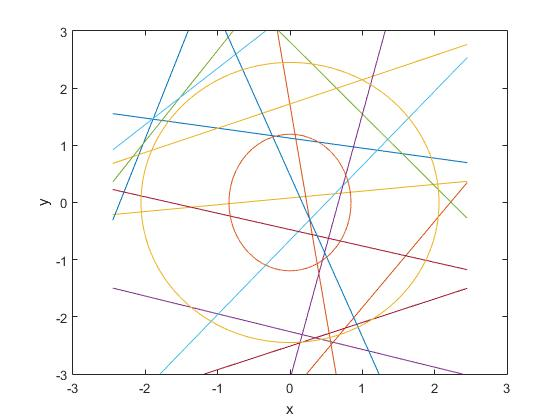
\includegraphics[width=60mm]{graf_primer.jpg}
\caption{Primer generiranih elips in premic \label{overflow}}
\end{figure} 

Na sliki 1 vidimo 2 elipsi generirani s funkcijo ``elipsa'' s parametroma $xmax=3$ in $ymax=3$ in 15 premic z naključnima parametroma $(p, \theta)$ kot opisano zgoraj. 

\subsubsection{Zamaknjene krožnice}

Za ponazoritev zamaknjenih krivulj sva se, iz praktičnih razlogov pri generiranju le-teh, odločila za krožnice. Funkciji ``kroznica\_zamaknjena'' sva podala parameter $rmax$, ki določa interval $(0,rmax)$, na katerem naključno določiva radij večjega kroga $r$. Nato znotraj kroga naključno generirava točko, podano s parom $(k,fi)$, kjer je $k$ oddaljenost od izhodišča, $fi$ pa kot, ki ga oklepata abcisa in krajevni vektor do naše točke. Radij manjše krožnice $rm$ generirava naključno na intervalu $(0,(r-k))$. Nato krožnici parametrizirava, na podoben način kot elipsi. $x$ kordinate množice točk so podane kot vektor $x = r*cos(t)$, $y$ kordinate pa kot vektor $y = r*sin(t)$, kjer je t vektor točk med 0 in $2\pi$ z razmikom 0.05. Manjšo krožnico parametrizirava na podoben način. Funkcija torej vrne matriki, kjer stolpca predstavljata $x$ in $y$ kordinate množice točk, ki opisujejo krožnici. 

\subsubsection{Splošna konveksna krivulja}
Splošni konveksni krivulji generirava s pomočjo dveh funkcij: ``random\_konveksna'' in ``notranja\_konveksna''. Prva dobi za parameter $j$, ki ponazarja število naključnih točk, ki jih bo funkcija generirala. Točke so podane z dvema vektorjema $a$ in $b$ dolžine $j$, ki vsebujeta naključna štvila na intevalu $[-0.5,0,5]$. Nato na teh dveh vektorjih pokličemo vgrajeno funkcijo ``convhull'', ki za podano množico točk vrne vektor indeksov točk $h$, ki razpenjajo  najmanjšo konveksno ovojnico, ki vsebuje vse točke, podane v argumentu. Funkcija torej na koncu vrne trojico vektorjev $a$,$b$ in $h$. Funkcija ``notranja\_konveksna'' pa deluje tako, da najprej iz vektorjev $a$ in $b$, ki ju vrne ``random\_konveksna'', odstrani elemente na mestih, ki so podani v vektorju $h$. Nato izmed preostalih točk naključno izbere 40 odstotkov le-teh in jih vrne kot vektorja $a1$ in $b1$. Na dani množici točk ponovno pokličeva funkcijo ``convhull'', rezultat pa shraniva kot $l$. Funkcija  ``notranja\_konveksna'' vrne trojico $a1,b1$ in $l$. Primer generiranih splošnih konveksnih krivulj je prikazan na sliki 2.

\begin{figure}[h]
\centering
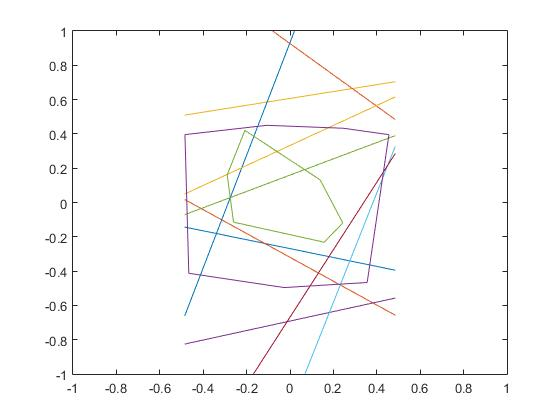
\includegraphics[width=90mm]{primer_konveksne.jpg}
\caption{Primer generiranih konveksnih krivulj in premic \label{overflow}}
\end{figure} 

\subsection{Implementacija algoritma}
Do sedaj sva napisala algoritme, ki so uspešno generirali elipse, krožnice, splošne konveksne krivulje in pa premice s parametrizacijo $(p, \theta)$. V naslednjem koraku sva želela dobiti algoritem, ki bo preštel, koliko naših premic seka večjo oziroma manjšo konveksno krivuljo. V ta namen sva iz spletnega portala MathWorks vzela funkcijo ``intersections'', ki prejme vektorje točk, ki opisujejo krivulji in vrne vektor $x$ koordinat presečišč. Ker je za najine potrebe dovolj preveriti, če se krivulji sekata, naju je bolj zanimala dolžina vrnjenega vektorja. To delo opravlja funkcija ``presecisca''. Na koncu sva poračunala še dolžini konveksnih krivulj in ju med seboj delila za primerjavo rezultatov. Za različne krivulje, se algoritem razlikuje minimalno. Funkcija, ki izvaja zgoraj opisani algoritem za primere splošnih krivulj, je prikazana spodaj.

\begin{figure}[h]
\centering
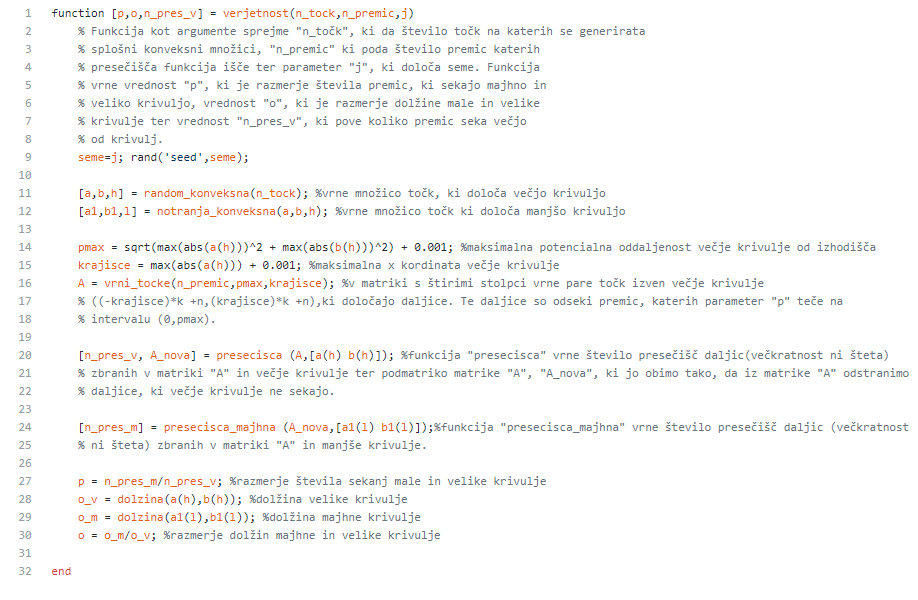
\includegraphics[width=110mm]{slika_kode}
\caption{slika kode v Matlabu \label{overflow}}
\end{figure}

\subsection{Analiza dobljenih rezultatov}
Če sva preko posameznega para konveksnih krivulj generirala več kot 300 premic, so bili rezultati že relativno blizu pričakovanim. Zato sva generirala 400 parov elips, krožnic in splošnih konveksnih krivulj ter za vsak par 1000 premic in na teh vhodnih podatkih poklicala najino glavno funkcijo (npr. ``verjetnost''). Rezultate sva shranila v matriko velikosti $400 \times 5$, ki po vrsticah prikazujejo posamezen poskus, po stolpcih pa razmerje obsegov, razmerje presečišč, absolutno razliko in predznačeno razliko med navedenima vrednostima ter število sekanja večje krivulje.
Zanimalo naju je tudi, kako hitra je konvergenca najine metode, oz. koliko premic je potrebno generirati za posamezen par elips, da bo rezultat razmeroma točen. Rezultate sva dobila tako, da sva za vsak par konveksnih krivulj primerjala absolutno razliko do točnega rezultata po vsakih 30 dodatnih premicah, pri čemer sva začela z desetimi, končala pa pri tisočih.


\subsubsection{Elipsa}
Povprečje absolutnih vrednosti razlike med razmerjem obsegov elips in razmerjem premic, ki sekajo eno in drugo elipso, je bila 0.0123, če pa dovolimo predznačeno razliko, se je v povprečju zmanjšala na 0.0012. Standardni odklon absolutnih razlik je bil 0.0098, delež premic, ki so sekale večjo krožnico pa v povprečju 0,783 \footnote[1]{Celotna tabela rezultatov je dosegljiva na github repozitoriju}. Rezultati se skladajo z najinimi pričakovanji, absolutna napaka je za to število premic relativno majhna.

Graf 4 prikazuje konvergenco metode na primeru elips.

\begin{figure}[h]
\centering
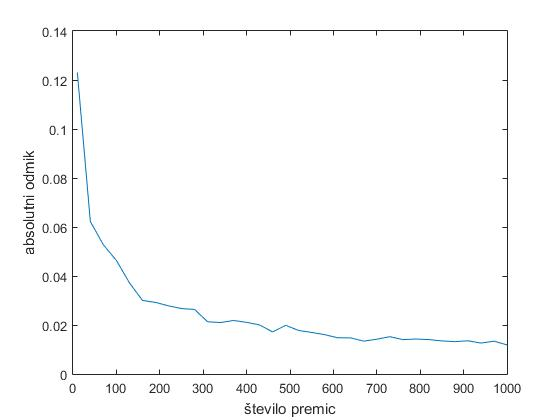
\includegraphics[width=80mm]{graf_elipsa2.jpg}
\caption{Graf napake v odvisnosti od števila premic za elipse \label{overflow}}
\end{figure} 

\subsubsection{Zamaknjena krožnica}

Povprečje absolutnih vrednosti razlike med razmerjem obsegov in razmerjem premic, ki sekajo eno in drugo krožnic je bila 0,0083, če pa dovolimo predznačeno razliko, se je v povprečju zmanjšala na 0,000053. Standardni odklon absolutnih razlik je 0,0074. Vse generirane premice so sekale večjo krožnico. V spodnjem grafu je prikazana povprečna absolutna razlika do točnega rezultata v odvisnosti od števila premic, ki sva jih generirala ob izvedbi eksperimenta.

\begin{figure}[h]
\centering
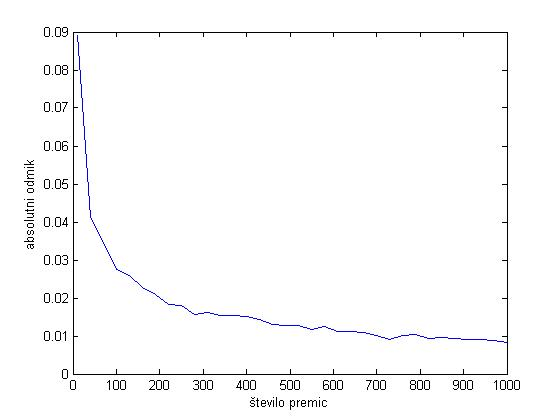
\includegraphics[width=80mm]{graf_kroznica.jpg}
\caption{Graf napake v odvisnosti od števila premic za krožnice \label{overflow}}
\end{figure} 


\subsubsection{Splošna krivulja}

Povprečje absolutnih vrednosti razlike med razmerjem obsegov in razmerjem premic, ki sekajo večjo in manjšo splošno konveksno krivuljo je bila 0,0117, če pa dovolimo predznačeno razliko, se je v povprečju zmanjšala na 0,00008. Standardni odklon absolutnih razlik je 0,0095. Delež premic, ki so sekale večjo krožnico je v povprečju 0,782. V spodnjem grafu je prikazan povprečna absolutna razlika do točnega rezultata v odvisnosti od števila premic, ki sva jih generirala ob izvedbi eksperimenta.

\begin{figure}[h]
\centering
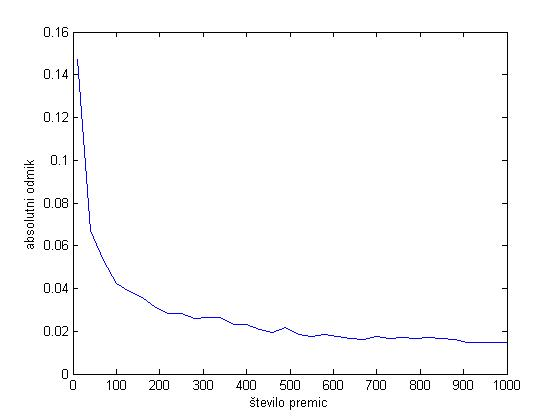
\includegraphics[width=80mm]{graf_splosna.jpg}
\caption{Graf napake v odvisnosti od števila premic za zasplošne krivulje \label{overflow}}
\end{figure} 

Iz grafov je razvidno, da se z večanjem premic vedno bolj približujemo pravemu rezultatu, vendar je konvergenca počasna. 

\section{Sklep}
Pri projektu sva se na dva načina prepričala o veljavnosti naše hipoteze: da je verjetnost sekanja manjše konveksne krivulje, če sekamo večjo, enaka razmerju dolžine obeh krivulj. Najprej sva ob naslanjanju na Cauchy-Crofton fromulo in definicijo pogojne verjetnosti podala idejo dokaza v teoretičnem smislu, v drugem delu pa sva izvedla še eksperiment, ki je hipotezo potrdili na konkretnih krivuljah. 
Ugotovila sva, da je konvergenca glavnega algoritma,ki primerja razmerje obsegov z razmerjem sekanj, odvisna od deleža premic, ki sekajo večjo krivuljo. To je najbolj očitno pri krožnicah, saj v tem primeru lahko paramater $p$ pri premicah omejimo kar na radij krožnice in tako zagotovimo, da bodo vse premice sekale vsaj večjo krožnico. Pri splošnih krivuljah je tako omejevanje parametra $p$ težje, zato se nekaj premic "izgubi" in je konvergenca počasnejša. 

Med izdelovanjem projekta sva ugotovila, da je ključnega pomena, da premice generiramo kot par $(p, \theta)$, kot je opisano v poglavju $3.2$. Hipotezo sva ob tej predpostavki potrdila. Za izboljšanje algoritma bi bilo smiselno spremeniti funkcijo ``intersections'', ki bi namesto koordinat presečišč preverjala samo, če se krivuljakrivulja in premica sekata. Tako bi lahko algoritem izvajali v hitrejšem času in rezultate preverjali z večjim številom premic. Kljub temu sva se z rezultati zelo približala teoretičnim vrednostim. Morda bi bilo prav tako smiselno tudi točke, okoli katerih sva generirala konveksno ovojnico, izbrati pod kakšnimi drugimi omejitvami, vendar verjameva, da to na rezultat ne bi smelo vplivati.

\end{document}
